\section{Agent Perspective}\label{sec:conceptional_view}

While previous sections described the agent's external environment and interactions, this section examines the internal structure of ACUs.
Here, we focus on two prevalent agent types: \emph{Foundation agents} (based on foundation models) and \emph{specialized agents} (based on domain-specific design).

\begin{description}
    \item[Foundation Agent:] \label{sec:foundation_agent}
    A foundation agent \citepeg{zheng_gpt-4vision_2024} uses a \emph{general pre-trained} foundation model (such as an LLM or VLM) as its policy $\pi$. While currently dominated by LLMs and VLMs, this category encompasses any architecture leveraging broad pre-training for zero-shot or few-shot transfer, including vision-language-action (VLA) models or diffusion models. These agents employ the model's broad knowledge and in-context learning capabilities for \emph{episodic improvement} (see \cref{sec:learning_strategy_pretraining,sec:episodic_improvement}).
    For example, a text-based foundation model receives a textual observation $o_t$ alongside a prompt specifying its role as agent, a description of available UI actions $\mathcal{A}$, and the instruction $i$. The model then \emph{generates} an action $a_t$ that is executed in the environment.
    %During each episode, the agent typically accumulates a \emph{history} of past observations and actions to provide additional contextual information to the foundation model as needed (see \cref{sec:agent_policy}).
    \item[Specialized Agent:] \label{sec:reinforce_agent}
    A specialized agent \citepeg{humphreys_data-driven_2022} employs a \emph{custom} network architecture as its policy $\pi$, which \emph{predicts} actions $a_t \in \mathcal{A}$ based on a given observation $o_t$ and instruction $i$, relying on the possibilities of the predefined output options.
    For example, the architecture might process an image $o_t$ and a text instruction $i$ as inputs through encoder networks and predict logits for each action type (such as \texttt{clicking}) alongside additional outputs (such as screen coordinates \texttt{(x,y)}). 
    %To track the past, observations are continuously aggregated in an internal Markov \emph{state}.
    Learning typically involves \emph{environment learning} techniques such as reinforcement learning (see \cref{sec:environment_adaption}).
\end{description}

Specialized agents work particularly well on narrow tasks and when the task conditioning of humans (the instruction) is limited (e.g., fill out a simple form given a user ID). In such cases, specialized agents often perform robustly and are computationally efficient due to their smaller parameter count \citepeg{humphreys_data-driven_2022}.
However, in multi-step tasks with diverse observation spaces or strong instruction-based conditioning, agents clearly benefit from general pre-training and reasoning techniques such as Chain-of-Thought (CoT) \citepeg{zhou_webarena_2024}. 

\Cref{table:two-main-agents} summarizes the key characteristics of the two common agent designs, highlighting their differences in architecture, action type, memory of information from past episodes, and learning strategy.

\begin{table}
    \caption{Properties of the two common ACU types.}
    \label{table:two-main-agents}
    \begin{tabular}{lllll}
    \toprule
   \textbf{ACU Agent Types } & \textbf{Architecture}   & \textbf{Action}  & \textbf{Memory}  & \textbf{Learning Strategy} \\ 
    \midrule
    Foundation agent & LLM / VLM               & Generation       & history-based  & General + Episodic \\
    Specialized agent  & Custom                  & Prediction       & state-based    & Environment learning  \\ 
    \bottomrule
    \end{tabular}
\end{table}

\subsection{Policy -- How to Act}\label{sec:agent_policy}
The policy $\pi$ defines how an agent selects actions \citep[Chapter~1.3]{sutton_reinforcement_2018}. For computer control, we distinguish three types of policies: Memoryless policies that act only on the current input; history-based policies that use explicit past observation and/or action sequences; and state-based policies that aggregate information about the past in an internal memory. 
%Among these, history-based and state-based policies leverage distinct types of memory to track past observations and/or actions.
Among them, history-based policies are the main research focus in the surveyed reviews, with almost $60$ out of the reviewed $87$ ACUs using some form of history in their policy (see Appendix \cref{fig:policy-dist} and \cref{tab:agent_literature}).
%The distribution of these policies across agents analyzed in this review shows in \cref{fig:policy-dist} (for a detailed association to publications, refer to \cref{tab:agent_literature}).

\subsubsection{Memoryless Policies}\label{sec:agent_policy_memoryless}
Memoryless policies \citepeg{chen_webvln_2024} ignore past observations and actions and act solely on the current observation $o_t$:
\begin{equation}
a_t \sim \pi(\ \cdot\ |\ o_t,\ i\ ) \label{eq:memoryless-policy}
\end{equation}

Memoryless policies are often insufficient for real-world control scenarios where context across time is critical and selecting an appropriate next action $a_t$ requires information about past observations $o_{t-n}, ..., o_{t-1}$ and/or actions $a_{t-n}, ..., a_{t-1}$. 
For instance, in the context of purchasing multiple items from an online store, an agent must remember which items were already added to the shopping cart.
% Therefore, state-of-the-art agents utilize more complex policies.
Still, since memoryless can be sufficient for specific tasks, their simplicity is sometimes leveraged in model design \citepeg{shvo_appbuddy_2021}.

\subsubsection{History-based Policies}\label{sec:agent_policy_history}
History-based policies track the past by adding observations and actions in a continuously growing sequence, called history $h_t=\left(o_{0},\hdots,o_{t-1},a_{0},\hdots,a_{t-1}\right)$ \citepeg{zheng_gpt-4vision_2024}.
For example, a vision-only agent's history consists of all the screenshots it perceived and the actions it performed during an episode. When predicting the next action $a_t$, the agent retrieves relevant information from its history $h_t$:
%
\begin{equation}
a_t \sim \pi(\ \cdot\ |\ o_t,\ i,\ h_t\ ) \label{eq:history-based-policy}
\end{equation}

Foundation agents commonly follow this pattern, as foundation models typically come with a context window to track past information, a specific instance of a policy history.
A key challenge with history-based approaches lies in the high dimensionality of observations $o_t$ (often screenshots or long textual descriptions). They either do not fit into the limited context windows of foundation models or, if they fit, they are computationally very expensive due to the large amount of required tokens.
Therefore, the history $h_t$ is often approximated as $h_t^*$. Common simplifications include:

\begin{description}
    \item[Actions only:] Keep only the past actions $h_t^*=\left(a_0,\hdots,a_{t-1}\right)$ and discard the observations \citepeg{zheng_gpt-4vision_2024}. In extreme cases, retain only the last action $h_t^*=\left(a_{t-1}\right)$ \citepeg{gao_assistgui_2024}.
    \item[Selective observations] Retain certain previous observations $o_{<t}$, such as keeping the last two screenshots with all actions as $h_t^*=\left(o_{t-2},o_{t-1},a_0,\hdots,a_{t-1}\right)$ \citep{furuta_multimodal_2024}.
    \item[Embedded summaries:] Create embeddings of the last observations $h_t^*=\left(\tilde{o}_{t-4},\hdots,\tilde{o}_{t-1},a_0,\hdots,a_{t-1}\right)$ \citep{lu_gui_2024}.
    \item[Text summaries:] Summarize past observations into text, enabling to keep the entire summarized observation history alongside raw actions $h_t^*=\left(\tilde{o}_{0},\hdots,\tilde{o}_{t-1},a_0,\hdots, a_{t-1}\right)$ \citep{zheng_synapse_2024}.
\end{description}

These strategies reduce token usage but risk omitting essential information, as the function for reducing information is not optimized for the given task. While suitable for simple GUIs, they are likely to limit performance in tasks requiring longer-term reasoning.

\subsubsection{State-based Policies}\label{sec:agent_policy_state}
In contrast, state-based policies rely on a compact internal memory $m_t$, often referred to as a Markov state, that is of fixed dimensionality and used during the action selection process \citepeg{humphreys_data-driven_2022}:
%
\begin{equation}
a_t \sim \pi(\ \cdot\ |\ o_t,\ i,\ m_t\ ) \label{eq:state-based-policy}
\end{equation}
%
This internal state $m_t$ is updated at each time step via a deterministic state-update function, typically of the form $m_{t+1}=f_m(o_{t},m_{t})$.
In practice, $f_m$ is commonly implemented as a learnable function, such as a recurrent neural network, enabling the agent to track task-relevant aspects of the history in a compressed representation for improved decision-making \citepeg{humphreys_data-driven_2022}.

While foundation models typically employ history-based policies, specialized agents often rely on state-based policies.
A notable exception is \citet{zhang_appagent_2023}, who propose a foundation agent with a state-based policy using an external \emph{text-based} state $m_t$. The foundation model not only generates the next action $a_t$ but also the next state $m_{t+1}$ given the current state $m_{t}$ and observation $o_t$, effectively operating as both policy and state-update function.

\subsubsection{Mixed Policies}\label{sec:agent_policy_mixed}
Mixed policies are hybrid approaches that combine history and state.
For example, \citet{bonatti_windows_2024} prompt their internal foundation model with the past actions and the last observation $h_t^*=\left(o_{t-1},a_0,\hdots, a_{t-1}\right)$, while keeping an external text-based state $m_t$.
Similarly, \citet{iki_berts_2022} feed the current observation $o_t$, the last action $h_t^*=\left(a_{t-1}\right)$, and an external text-based state $m_{t}$ into a fine-tuned model to predict the next action $a_t$ as well as state $m_{t+1}$.

% Zhang et al. \cite{zhang_appagent_2023}, use a foundation, state-based agent. Their foundation model generates the next action and a text-based summary given the current observation $o_t$ and the previous summary; the summary is essentially a text-based state.

\subsubsection{Recommendations}
Most state-of-the-art approaches leverage foundation models that use history-based policies.
Nevertheless, processing the full, unfiltered episode history at every decision step is computationally inefficient and, in many cases, infeasible. This limitation necessitates some form of history simplification for history-based policies. 
A common approach involves retaining only past actions while discarding observations. Although effective for current benchmarks, this method deliberately omits observation information that is essential for solving more complex tasks requiring reasoning over temporally distributed observations.

Other history simplification strategies are either manually crafted \citepeg{cho_caap_2024} or based on generic summarization models \citepeg{zheng_synapse_2024}, both lacking adaptability to environments.
We posit that the ability to act effectively in complex environments inherently involves the capacity to learn what historical information is relevant and what can be safely ignored. Therefore, we argue that \textbf{history simplification should be a learnable component of the agent}, integral to achieving robust and generalizable behavior for complex tasks. The literature on \emph{world models} is herein closely related (cp. \citet{ha2018world}, \citet{lecun_path_2022}, \citet{hafner2025mastering}).

Notably, specialized agents employ state-based policies, wherein past information is compressed into a Markovian state via a learnable state-update function.
This function can be interpreted as a form of learned history simplification.
This conceptual link between specialized and foundation agents, revealed by our taxonomy, may inspire future history simplification research for foundation agents.


\subsection{Learning Strategy - How to Learn to Act}\label{sec:learning_strategy}

An agent’s learning strategy can involve up to three stages (not all ACUs utilize every stage):

\begin{description}
    \item[General pre-training:] 
        The agent acquires broad, environment-agnostic knowledge. Examples include foundation models learning general-purpose capabilities or vision backbones learning image representations.
    \item[Environment learning:] 
        The agent learns to adapt to a specific computer environment. This involves explicit parameter (weight) updates or implicit methods, such as storing environment experiences for later retrieval.
    \item[Episodic improvement:] 
        The agent refines its performance within the current episode through methods such as instruction tuning or few-shot learning \citep{brown_language_2020}. Unlike the previous steps, this step does not result in persistent learning, as changes are discarded post-episode.
\end{description}

\Cref{fig:learning-flow} illustrates how these steps sequentially combine into learning strategies for both foundation and specialized agents.
Our analysis of learning strategies shows that the combination of general pre-training with prompting is the most common strategy (see Appendix~\Cref{fig:learning-strategy-dist}).
The following sections explore each learning step in detail, emphasizing current practices and highlighting exceptions.

\begin{figure}[t]
    \centering
    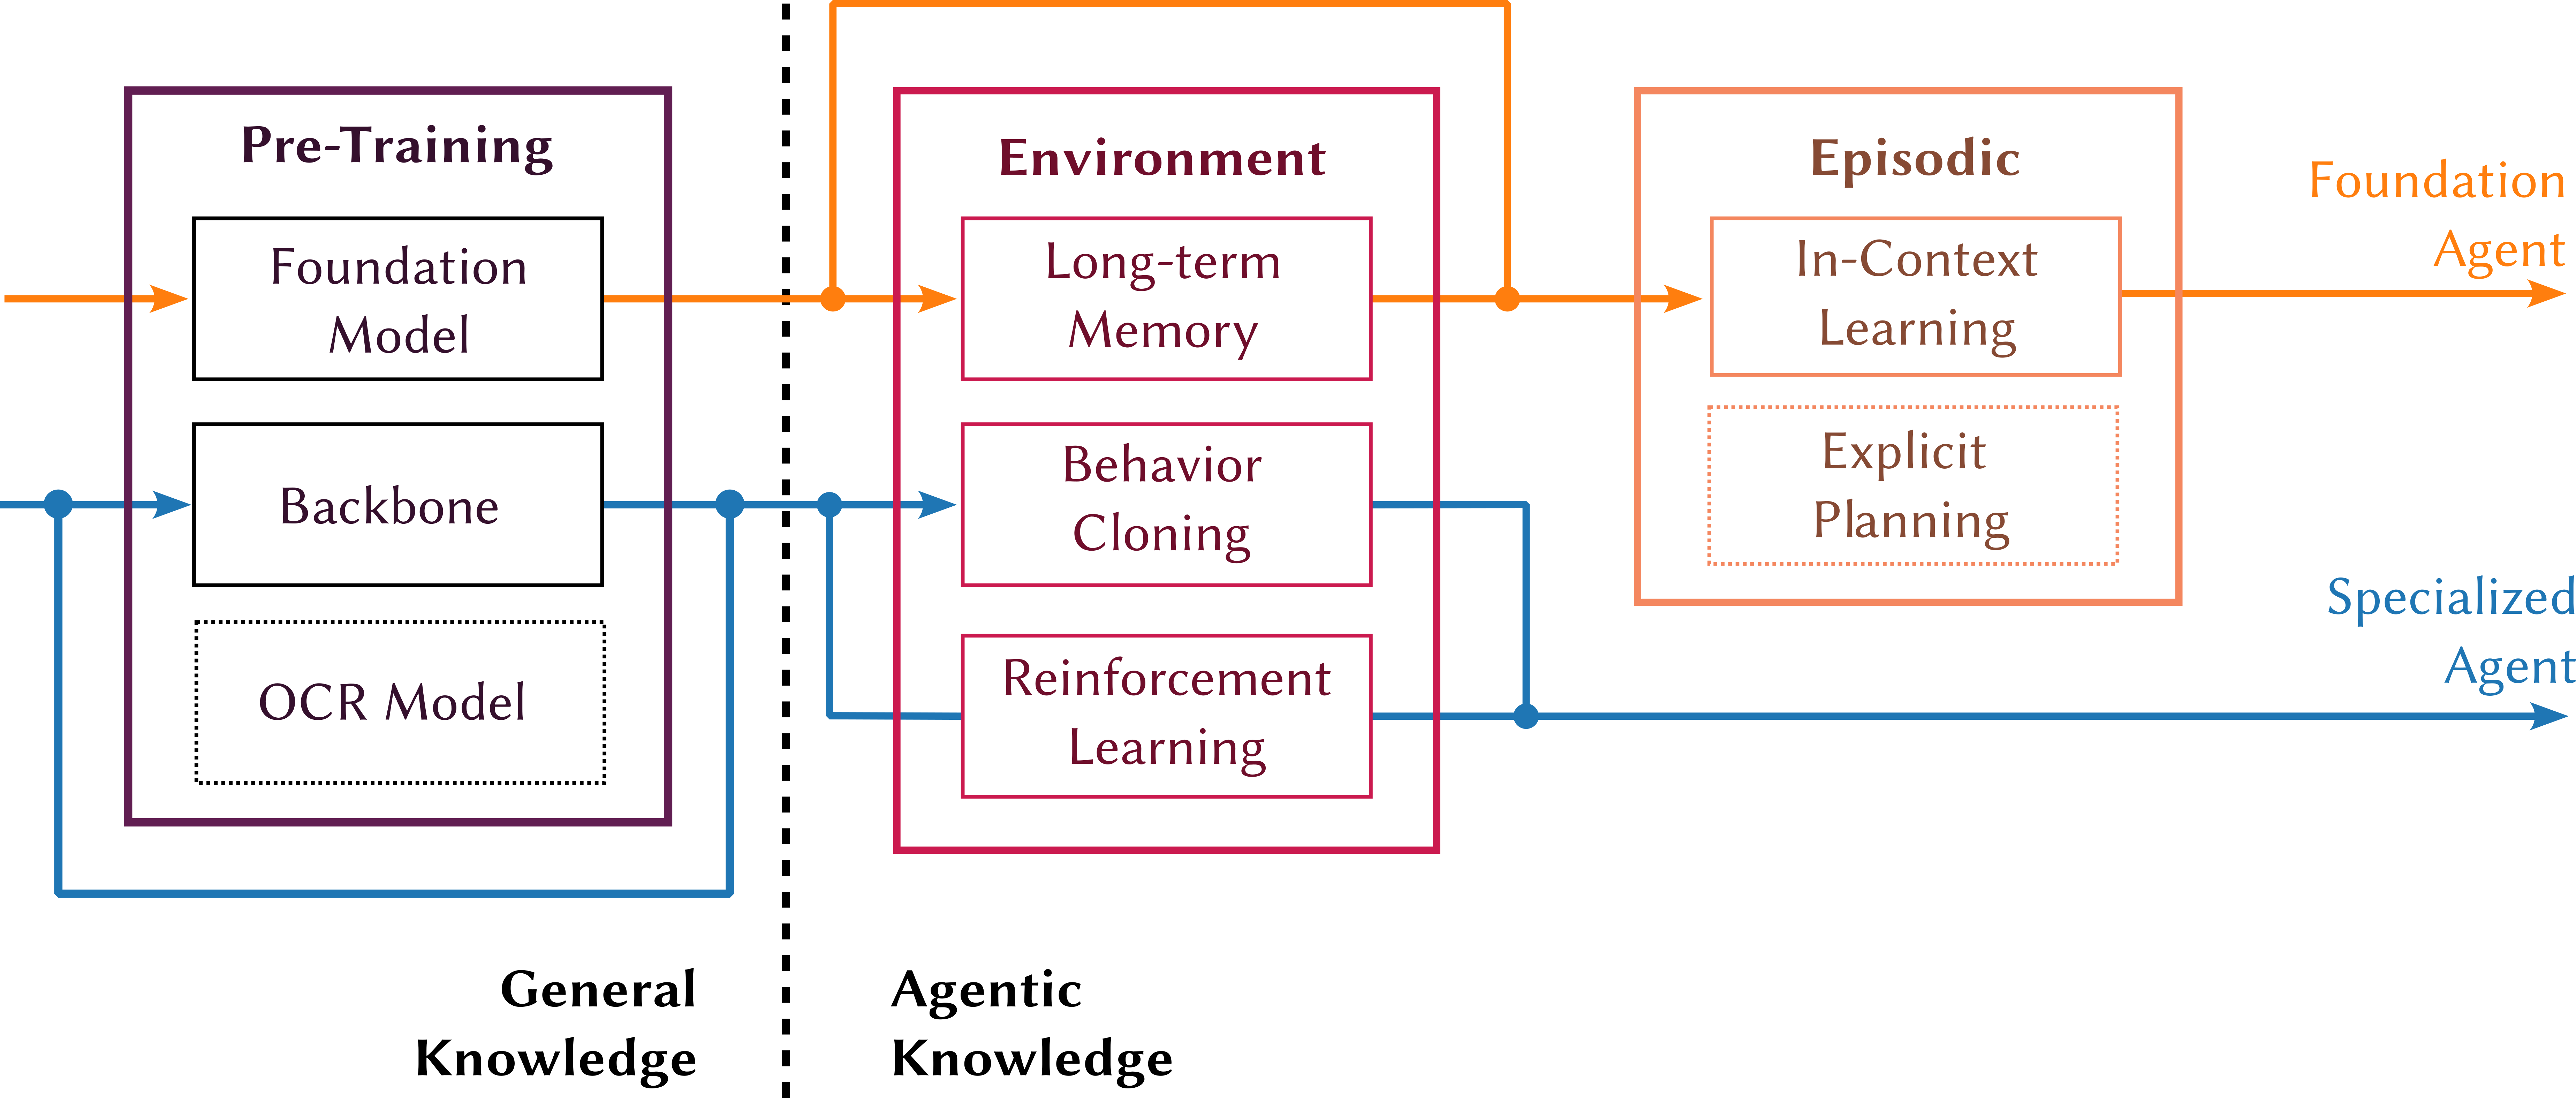
\includegraphics[width=0.95\linewidth]{figures/learning_flow_colored.png}
    \caption{Overview of learning steps and strategies: \emph{Pre-training} involves acquiring broad, environment-agnostic knowledge. \emph{Environment learning} and \emph{episodic improvement} hone a ACU's agentic capabilities. A combination of these steps defines a learning strategy. ACUs typically follow one of two strategies: (1) \emph{Specialized agents} (blue)  start from scratch or use a pre-trained backbone, learn to act in a specific environment through behavioral cloning (BC) or reinforcement learning (RL) ; (2) \emph{foundation agents} (orange) begin with a general-purpose foundation model, optionally storing successful episodes for future demonstration retrieval, and employ in-context learning.}
    \Description{The diagram depicts the learning strategies and typical training pathways of agents for computer use, organized into three main stages arranged from left to right: pre-training, environment learning, and episodic improvement. The pre-training stage includes the foundation model, backbone, and OCR model components and corresponds to general knowledge acquisition. The environment learning stage involves long-term memory, behavior cloning, and reinforcement learning, which together form agentic knowledge. The episodic improvement stage consists of in-context learning and explicit planning, aimed at refining agent performance in specific tasks. Two main learning strategies are illustrated by color-coded flow paths: foundation agents begin with the foundation model, optionally leverage components in the environment stage, and utilize in-context learning during episodic improvement, while specialized agents start from the backbone model or from scratch and rely on behavior cloning or reinforcement learning during environment learning. A dashed vertical line separates the pre-training phase from the subsequent stages, highlighting the transition from general to agentic knowledge. The figure emphasizes that foundation and specialized agents generally follow distinct and limited combinations of these training strategies.}

    \label{fig:learning-flow}
\end{figure}

\subsubsection{Leveraging General Pre-Training} \label{sec:learning_strategy_pretraining}
General pre-training serves as an initialization stage for an agent. This initial knowledge can be modified and adapted through \emph{environment learning} (e.g., fine-tuning, see \cref{sec:environment_adaption}) or preserved and utilized via \emph{episodic improvement} (e.g., prompting, see \cref{sec:episodic_improvement}).

Foundation agents primarily rely on the former approach. They leverage foundation models with broad knowledge and in-context learning capabilities \citep{brown_language_2020}. These capabilities can eliminate the need for environment-specific fine-tuning, allowing agents to operate in computer environments using only the foundation model's broad knowledge and instructions provided through prompts to adapt to specific environments \citepeg{kim_language_2023}.
For example, GPT-4 \citep{openai_gpt-4_2024}, when prompted as a web agent, can complete tasks such as filling out forms or navigating website links \citep{zheng_gpt-4vision_2024}.

In contrast, specialized agents are either trained from scratch \citepeg{humphreys_data-driven_2022} or initialized with a pre-trained backbone (e.g., an image encoder) to accelerate learning the observation space \citep{li_mug_2024}. These agents typically require additional fine-tuning to adapt to computer environments (see \cref{sec:environment_adaption}).
% 
The foundation model or backbone choice depends on the observation space, action space, and specific task requirements. For example, 
%\begin{itemize}
    %\item 
    \citet{zheng_gpt-4vision_2024} use GPT-4 \citep{openai_gpt-4_2024} as a multi-modal foundation model for their bi-modal agent.
    %\item 
    \citet{gur_real-world_2024} employ a coding-proficient foundation model \citep{chung_scaling_2022} to generate executable code.
    %\item 
    \citet{shaw_pixels_2023} fine-tune a vision backbone for their vision-based agent.
    %\item 
    \citet{iki_berts_2022} fine-tune a text backbone for their text-based agent.
    %\item 
    \citet{song_visiontasker_2024} use pre-trained object detection and OCR models to convert screenshots into text-based observations for direct UI access actions.
    %\item 
    \citet{gur_real-world_2024} pre-train an LLM from scratch only on HTML data while utilizing an HTML-specific local and global attention mechanism.
%\end{itemize}

\subsubsection{Environment Learning}\label{sec:environment_adaption}
Environment learning involves adaptation to computer environments through experience. Three main approaches are used: \emph{reinforcement learning}, \emph{behavioral cloning}, and \emph{long-term memory}. Among them, behavioral cloning is the most frequently used strategy (see Appendix~\Cref{fig:environment-adaption-dist}). 

Many foundation agents bypass the environment learning step, relying solely on their pre-trained, out-of-the-box capabilities by using prompting strategies. While these capabilities can be remarkably effective \citepeg{zheng_gpt-4vision_2024}, the absence of environment learning limits these agents, as they lack mechanisms to adapt or improve their performance within specific computer environments.

\paragraph{Reinforcement Learning} \label{sec:environment_adaption_rl}

In reinforcement learning (RL), an agent acts in an environment and learns to maximize a cumulative reward by trial and error \citep{sutton_reinforcement_2018}.
For computer use tasks, such environments are hand-crafted simulations, called \emph{controlled environments}, designed to mimic real-world computer settings while providing a reward signal for guidance.
% 
RL has been implemented with various algorithms, including approximate policy iteration \citep{humphreys_data-driven_2022}, policy gradients \citep{shi_world_2017}, and bootstrapping with tree search \citep{shaw_pixels_2023}.

Agents in simpler environments may rely on brute-force exploration to learn directly from random behavior \citepeg{toyama_androidenv_2021, shvo_appbuddy_2021}.
However, in most computer environments, rewards are sparse as they are only given upon completing the assigned instruction $i$ \citepeg{shi_world_2017}, such as submitting a flight booking form after filling out \emph{all} details correctly.
Sparse rewards make learning from an initial random behavior often unsuccessful, as an agent is unlikely to predict a long action sequence by random chance \citep{humphreys_data-driven_2022}.
One strategy to mitigate sparse rewards is to begin by training an agent on human-labeled demonstrations (behavioral cloning), providing it with enough competence to start finding and learning from rewards \citepeg{shi_world_2017, humphreys_data-driven_2022}.
Relatedly, \citet{liu_reinforcement_2018} use human-labeled demonstrations to constrain the action space by defining sets of valid actions based on similarity to demonstrated actions, increasing the likelihood of reward discovery.

Without demonstrations, reward shaping \citep{ng1999policy} can artificially reduce sparsity by providing intermediate guidance, as shown by \citet{gur_learning_2019} and \citet{li_glider_2021}.
Alternatively, the task complexity can be adaptively adjusted. \citet{gur_environment_2021}, for instance, introduce a controlled environment that enables autonomous curriculum learning \citep{bengio2009curriculum} by automatically changing a task's complexity. Similarly, \citet{gur_learning_2019} employ curriculum learning by gradually moving an agent's starting point away from the goal state as it gains competence.

The key advantage of RL is its ability to autonomously explore environments and effectively navigate a dynamic dataset. However, RL's reliance on controlled environments limits its application to broad computer use tasks, as rewards must be defined and action consequences suppressed (i.e., ensure that actions within the simulation have no real-world consequences). The development of such environments can be very tedious, typically preventing current ACUs from acquiring broad knowledge by solely using RL.
Nevertheless, AndroidEnv \citep{toyama_androidenv_2021} combats this limitation by simulating a complete, virtual Android environment on top of which tasks can be configured by defining instructions and rewards.


\paragraph{Behavioral Cloning}\label{sec:environment_adaption_bc}

In behavioral cloning (BC) \citep{pomerleau_alvinn_1988}, an agent learns to mimic a shown behavior through supervised learning.
The shown behavior is usually a sequence of recorded observations and actions of a human completing a computer use task given an instruction \nolinebreak$i$.

Unlike RL, learning via BC does not require the agent to execute actions in the environment, making it applicable in \emph{uncontrolled} environments (trained based on observation-action pairs instead of a simulation). 
For example, \citet{zhang_you_2024} fine-tune a model on Android demonstrations from the work of \citet{rawles_android_2023}, while \citet{hong_cogagent_2024} combine Android demonstrations provided by \citet{rawles_android_2023} with Web demonstrations taken from the work of \citet{deng_mind2web_2023}.

BC methods vary in training strategies and data collection.
For example, \citet{gur_understanding_2023} train the entire model, \citet{hong_cogagent_2024} only update specific components, while \citet{li_effects_2024} use low-rank adaption \citep{hu_lora_2021} to fine-tune a foundation model.
Datasets are typically human-labeled \citepeg{humphreys_data-driven_2022}, but autonomous data collection methods also exist. For instance, \citet{furuta_multimodal_2024} use rejection sampling to identify successful trajectories from another agent's actions in a controlled environment, leveraging the environment’s rewards for validation. Similarly, \citet{lai_autowebglm_2024} iteratively collect successful demonstrations for improving their agent.

While BC can be used independently to train ACUs, it can also be used as a pre-trained step, with the ACU being fine-tuned afterward using RL to improve performance.
Typically, RL further enhances the agent by exploring aspects missing from the behavioral data. For instance, \citet{humphreys_data-driven_2022} demonstrate that after training their agent on $2.4$ million human-labeled actions, RL increases the task success rate from approximately $30\%$ to over $95\%$. 
Nonetheless, some agents rely entirely on BC, which can suffice for simpler tasks \citepeg{gur_understanding_2023}.

\paragraph{Long-Term Memory} \label{sec:environment_adaption_ltm}

\begin{figure}[b]
  \begin{subfigure}{0.49\linewidth}
    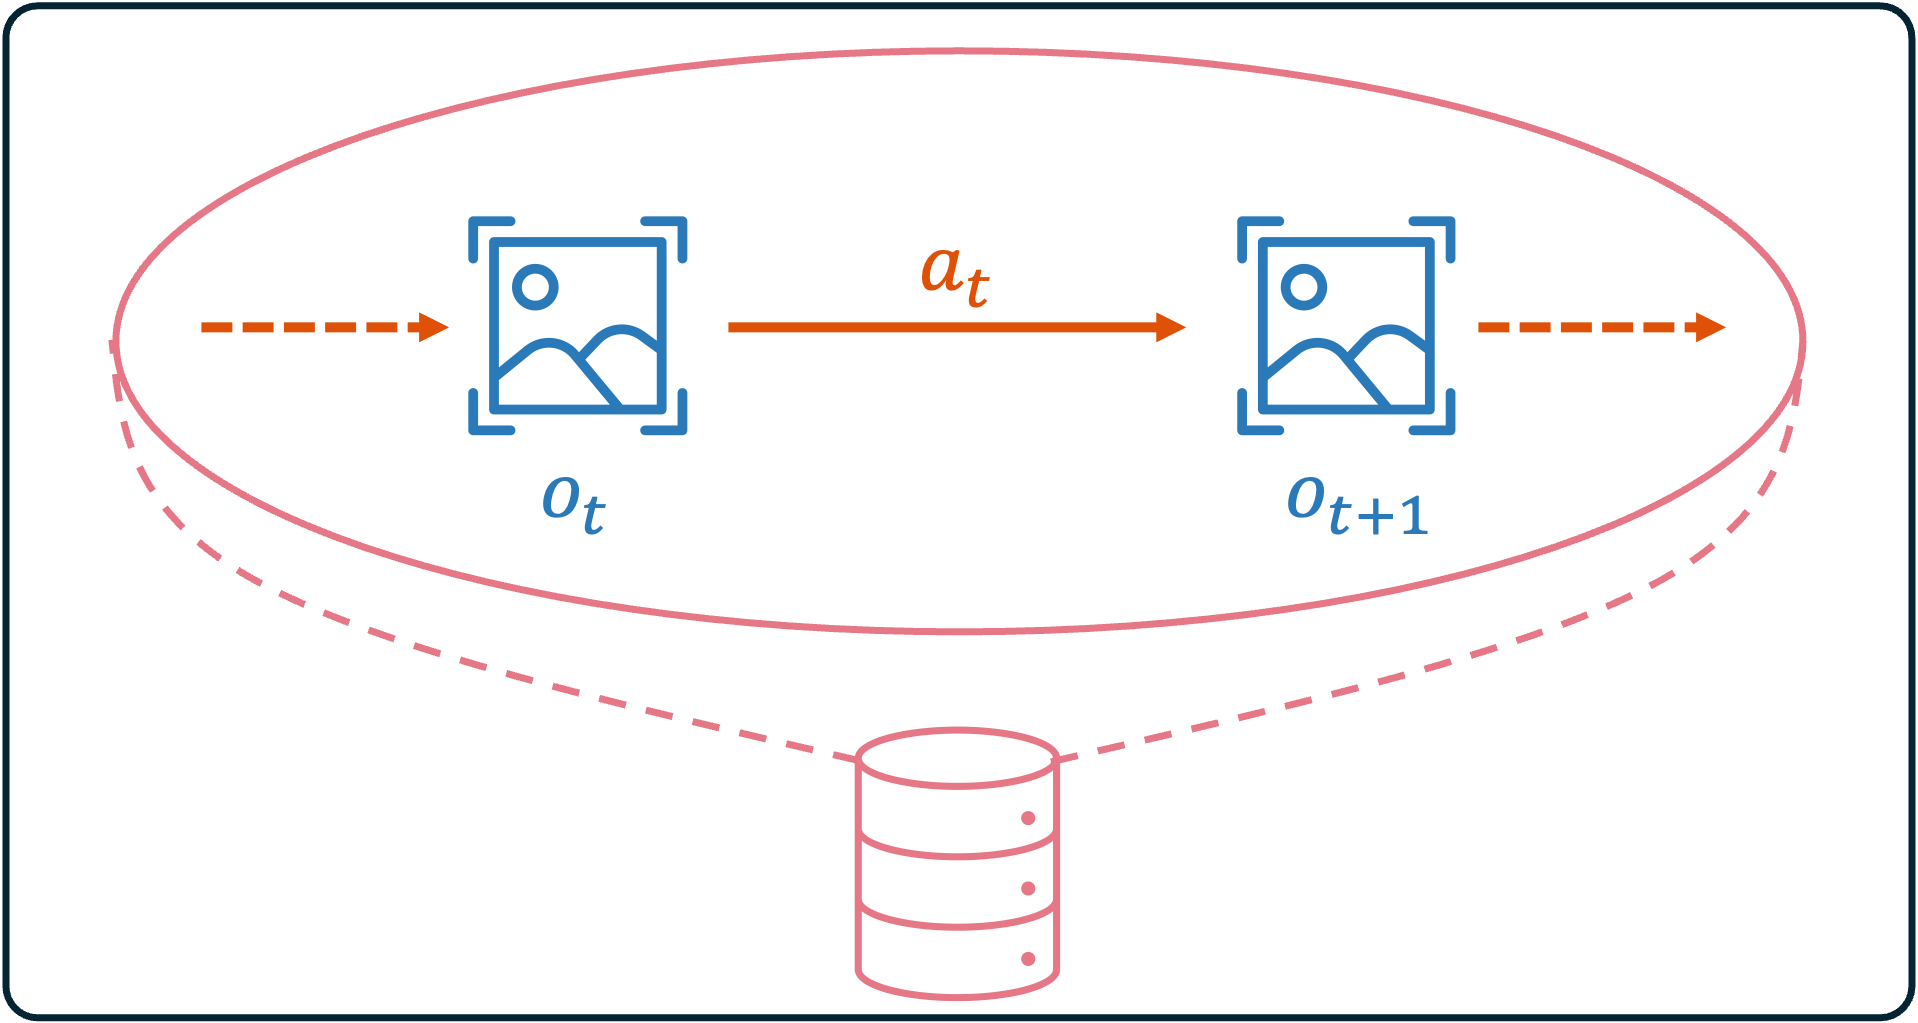
\includegraphics[width=\linewidth]{figures/few_shot_what_env.png}
    \caption{Memorize transitions $(o_t,a_t,o_{t+1})$}
    \label{fig:few_shot_what_env}
  \end{subfigure}
  \hfill
  \begin{subfigure}{0.49\linewidth}
    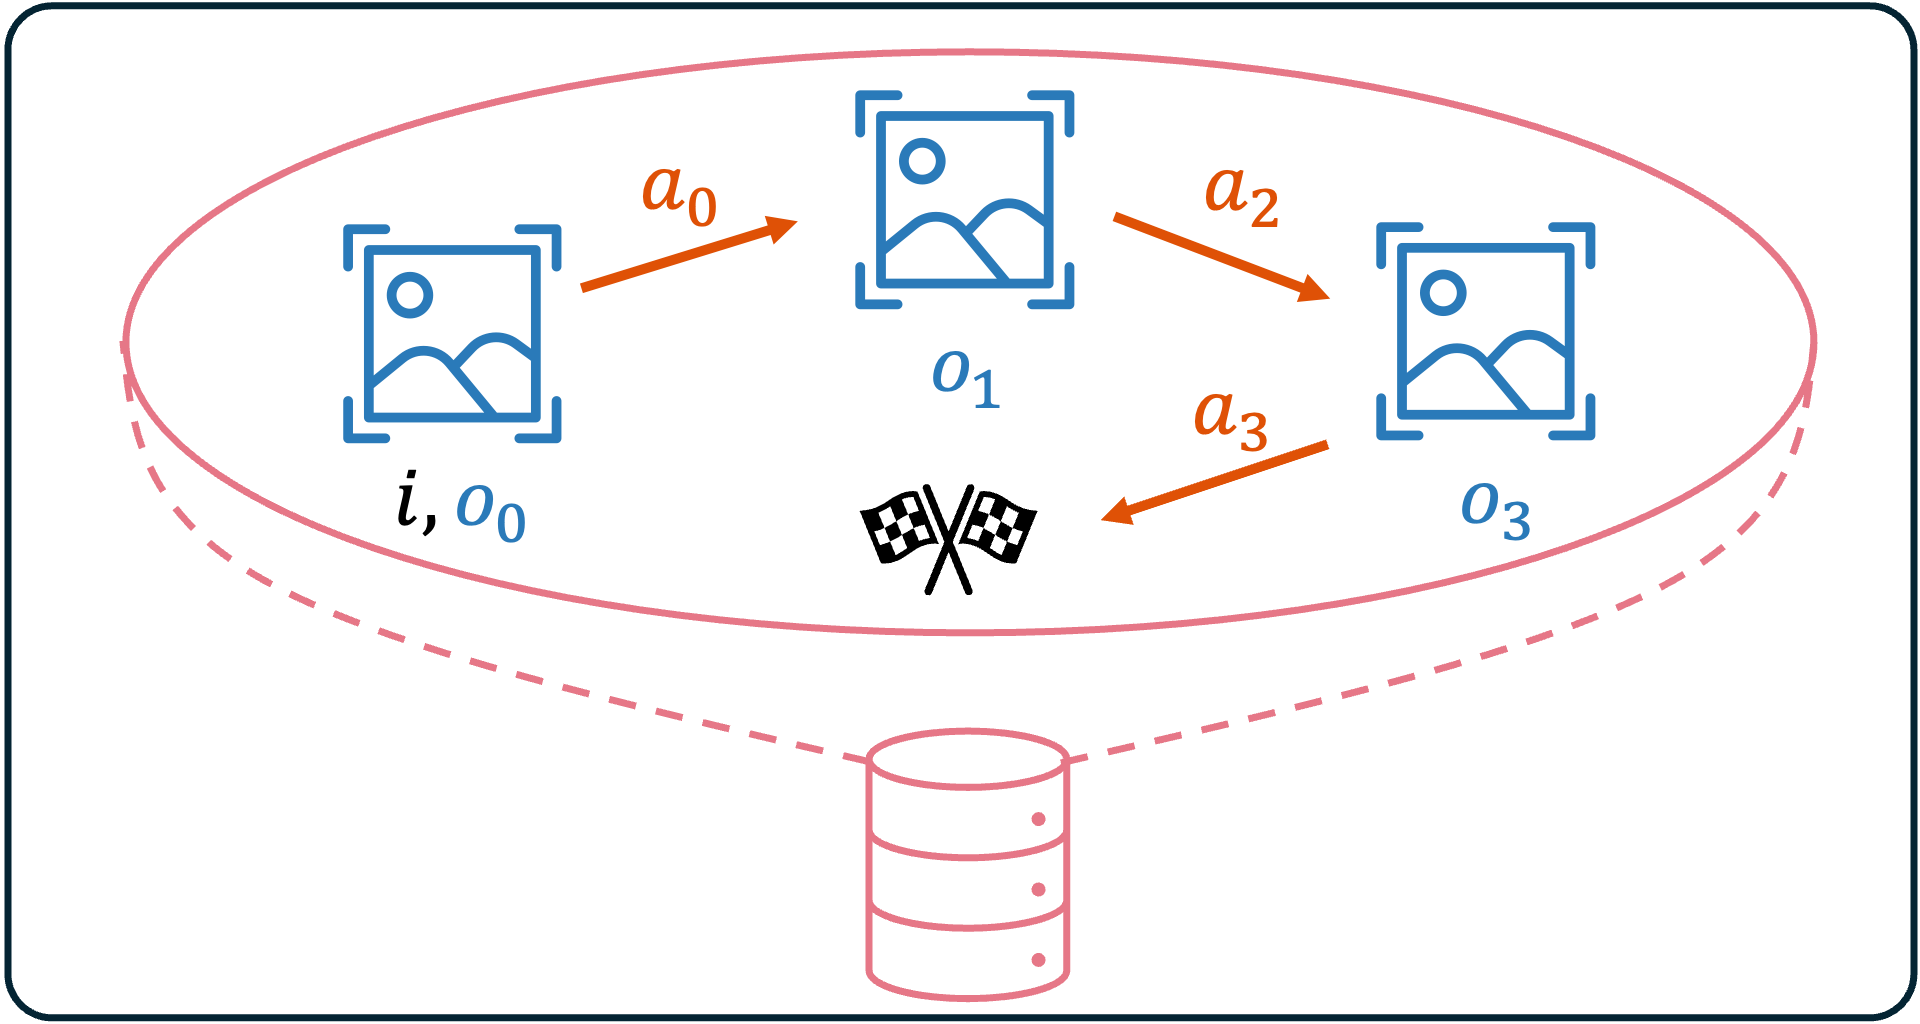
\includegraphics[width=\linewidth]{figures/few_shot_what_act.png}
    \caption{Memorize task demonstrations $(i,\tau)$}
    \label{fig:few_shot_what_act}
  \end{subfigure}
    \caption{Two kinds of experiences an agent can store in its long-term memory. (a) The agent memorizes the pre- and post-action observations as environment transitions $(o_t, a_t, o_{t+1})$. (b) The agent memorizes an instruction with a successful action-observation episode $(i, \tau)$}.
    \Description{This figure illustrates two conceptual approaches an agent can use to store experiences in long-term memory. The left panel shows storage of individual environment transitions as triplets consisting of the observation at time $t$, the action taken at time $t$, and the subsequent observation at time $t+1$. This emphasizes storing atomic transitions as discrete records. The right panel depicts storage of complete task trajectories, where an instruction is paired with the entire sequence of observations and actions from a successful episode. The figure uses a database symbol to represent the memory storage, highlighting that the left stores isolated transitions while the right stores full episodic trajectories.}
    \label{fig:few_shot_what}
\end{figure}

Foundation models exhibit strong few-shot learning capabilities \citep{brown_language_2020}, enabling foundation agents to enhance action prediction by incorporating successful demonstrations as examples directly into their context (see \cref{sec:episodic_improvement}).
This paradigm is also known as in-context learning (ICL).
Long-term memory extends ICL by first allowing the agent to execute and store successful trajectories in an external memory, and then later retrieve previous trajectories from this memory as examples of how a specific (sub-)task can be solved.
Importantly, since the examples are collected by the agent itself rather than provided by a human, the agent learns to improve its capabilities over time and adapts \emph{autonomously} to an environment (we discuss human prompt designs in the next section).
\cref{fig:few_shot_what} illustrates the two main types of experiences:

\begin{description}
    \item[Environment transitions:] 
        The agent memorizes environment transitions as triples ($o_t$, $a_t$, $o_{t+1}$), where $a_t$ represents the action taken, and $o_t,o_{t+1}$ capture the pre- and post-action observations, respectively. For example, the agent might store the consequence of its actions, such as ``clicking on the calculator app ($a_t$) on the home screen ($o_t$) opens the calculator app ($o_{t+1}$).'' \citet{wen_autodroid_2024} collect such transitions for Android apps in an offline phase by random exploration. They describe and summarize these transitions using an LLM, enabling the agent to enrich actionable elements with outcome information. For example, a \texttt{more options} button could be annotated to reveal specific hidden menu items, informing the agent what to expect if this button is clicked. Autonomous transition memories can also be combined with human demonstrations, as shown by \citet{zhang_appagent_2023} and \citet{li_appagent_2024}.
    \item[Task demonstrations:] 
        The agent memorizes task demonstrations by storing a tuple ($i$, $\tau_i$) containing the instruction $i$ and a successful demonstration $\tau_i=(o_{0},a_{0},\hdots,o_{t},a_{t})$ of solving $i$. Since only successful attempts are informative for the agent, the agent must have a mechanism to filter \emph{successful} trajectories. 
        % A common approach is to use a controlled environment's reward \citepeg{tao_webwise_2023} or human data \citepeg{li_appagent_2024}. Another approach is to use a foundation model to predict success \citepeg{}. 
        A common approach is to use a controlled environment's feedback and only to store trajectories that yield a high reward \citepeg{tao_webwise_2023}.
        To manage memory constraints, trajectories $\tau_i$ are typically simplified to $\tau_i^*=(\tilde{o}_0,a_0,\hdots,\tilde{o}_t,a_t)$ (where $\tilde{o}_i$ is a simplification of $o_i$) before being stored. 
        For instance, \citet{deng_multi-turn_2024} only keep the actions $\tau_i^*=(a_0,\hdots,a_t)$, while \citet{sun_adaplanner_2023} store the complete executable program that solves $i$.
        These simplifications mirror history simplifications ($h_t \rightarrow h_t^*$), as the history $h_t$ is a (partial) trajectory.
        An alternative approach for discovering successful trajectories is programming by demonstration. Here, a human supervises the agent, intervenes if necessary, and demonstrates the correct solution for $i$, enabling online learning. \citet{song_visiontasker_2024} propose this method to summarize the corrected behavior for future retrieval.
\end{description}

A limitation of memory-based approaches is their reliance on storing specific instances rather than learning abstract generalizations. To mitigate this, \citet{lee_explore_2023} organize memories into a graph where observations are nodes, actions are edges, and both are generalized to unify related experiences. For example, an action $a=$ \texttt{click(text=Bob)} is generalized to $a^*=$ \texttt{click(text=[contact name])}. When retrieving memories, the graph is searched, and parameterized actions are instantiated based on the current state $(o_t, i)$, grounding parameters like \texttt{[contact name]} to specific values.
However, it still remains challenging to map specific trajectory instances to general concepts and to later retrieve and adapt helpful general concepts for specific tasks.


\subsubsection{Episodic Improvement}\label{sec:episodic_improvement}
Episodic improvement refers to an agent's ability to enhance its performance within a single episode by reasoning over its current context, without retaining knowledge across episodes. This effectively trades test-time computing for improved task execution.

Foundation agents commonly achieve episodic improvement through in-context learning \citep{brown_language_2020}.
ICL encompasses techniques such as \emph{instruction tuning}, where guidance is provided to the model through the prompt, and few-shot learning, which gives examples of successful trajectories as \emph{demonstrations} to the agent.

In contrast, current specialized agents typically do not employ episodic improvement. However, analogous mechanisms exist, such as search-based planning in game-playing agents, which simulate future outcomes to guide action selection \citep{silver_mastering_go_2017}. Such approaches can be considered as a more traditional reasoning within agents.

\paragraph{In-Context Learning through Instruction Tuning} \label{sec:episodic_improvement_instruction}

Foundation models are often adapted to specific tasks through \emph{prompt engineering}.
Typically, these prompts are designed by humans to adapt a foundation model to specific environmental conditions \citepeg{zheng_gpt-4vision_2024} and can include guidance on valid actions, previous history, assumed roles, or intermediate reasoning steps.
\Cref{tab:in-context-learning} exemplifies some snippets taken from the (much longer) prompts in the literature (for more details, refer to Table 6 in Zheng at al.~\citep{zheng_gpt-4vision_2024}). 

While most prompts are human-authored, some methods automate prompt construction.
For example, \citet{sun_adaplanner_2023} uses a second model as a planner to autonomously generate prompts for the agent.
This strategy, known as \emph{self-prompting}, involves using multiple instances of the foundation model, each fulfilling different roles and interacting with one another through iterative prompting \citepeg{song_mmac-copilot_2024}.

With the rise of vision-language models, \emph{visual prompt engineering} has emerged. This includes techniques such as extending screenshots to incorporate user instructions \citep{lee_pix2struct_2023}, overlaying bounding boxes on actionable UI elements \citepeg{bonatti_windows_2024}, and adding unique identifiers for visual grounding \citepeg{zhang_ufo_2024}.

\begin{table}

    \caption{Example snippets of actual prompts.}
    \label{tab:in-context-learning}
     {\footnotesize
    \begin{tabular}{>{\raggedright\arraybackslash}p{3.5cm} >{\raggedright\arraybackslash}p{10cm}}
        \toprule
        \textbf{Category} & \textbf{Prompt Snippet} \\
        \midrule
        Action Generation & \texttt{[...] you can \textbf{click an object} by referring to its id, such as 'click id=..., [...]'} \citep{li_zero-shot_2023} \\ 
        %\hline
        Provide history $h_t$ &  \texttt{\textbf{Previous} Actions: \{PREVIOUS ACTIONS\}} \citep{zheng_gpt-4vision_2024} \\ 
        %\hline
        Prescribe a role & \texttt{Imagine that you are \textbf{imitating humans} doing web navigation [...]} \citep{zheng_gpt-4vision_2024} \\ 
        %\hline
        Elicit intermediate thoughts & \texttt{[...] \textbf{think about} what the current webpage is [...] analyze each step of the previous action history [...] based on your analysis [...] decide on the following action [...]} \citep{zheng_gpt-4vision_2024} \\ 
        %\hline
        Provide general guidelines & \texttt{To be successful [...] only issue a \textbf{valid action} [...] only issue \textbf{one action} [...]} \citep{zheng_gpt-4vision_2024} \\
        \bottomrule
    \end{tabular}
    }
\end{table}

\paragraph{In-Context Learning through Demonstrations}\label{sec:episodic_improvement_demostrations}

Few-shot learning enhances agent performance by providing example trajectories, ${\tau_1, \tau_2, \hdots}$, which demonstrate successful task execution.
\Cref{fig:few_shot} illustrates four common techniques for collecting and providing demonstrations to the agent. These common sourcing strategies include:

\begin{description}
    \item[Human-crafted:] 
        For a given class of tasks, a fixed set of human-crafted demonstrations $\{\tau_1, \tau_2, \hdots\}$ is provided to the foundation model \citepeg{kim_language_2023}.
    \item[Semantic retrieval:] 
        Based on the semantic similarity of the instruction $i$ compared to previous instructions, an agent retrieves human-crafted demonstrations from a database \citepeg{cho_caap_2024}.
    \item[Auxiliary model:] 
        A secondary agent is first used to generate a large set of demonstrations, after which the agent retrieves those demonstrations that are semantically relevant to the current instruction $i$.
    \item[Agent-collected:] 
        The agent autonomously collects its own demonstrations, referred to as \textit{long-term memory}, by searching through its past experiences (\cref{sec:environment_adaption_ltm}).
\end{description}

Given the limitations of context length, a provided trajectory $\tau = \bigl((o_0,a_0), (o_1, a_1), ... \bigr)$ is typically compressed $\tau \rightarrow \tau^*$,  analogous to history simplification ($h_t \rightarrow h_t^*$, \cref{sec:agent_policy_history}).

In addition to the trajectory, a demonstration may include rationales for each action taken \citepeg{cho_caap_2024}. These rationales, inspired by chain-of-thought prompting \citep{liu_chain_2023}, can aid the agent when making similar decisions. Such reasoning can be written by humans \citepeg{wang_enabling_2023} or generated autonomously by another model \citepeg{cho_caap_2024, sodhi_heap_2023}.

\begin{figure}[b]
    \centering
    %\centering
    % \includegraphics[width=1.0\textwidth]{figures/few_shot.png}
 \begin{subfigure}{0.49\linewidth}
    \centering
    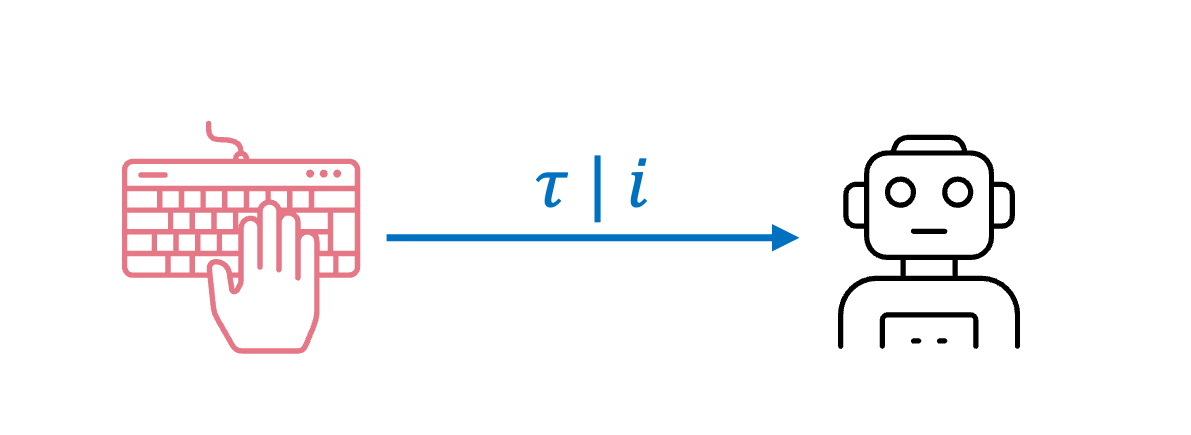
\includegraphics[width=0.7\linewidth]{figures/few_shot_1.png}
    \caption{Human-crafted.}
    \label{fig:few_shot_1}
  \end{subfigure}
  \hfill
  \begin{subfigure}{0.49\linewidth}
    \centering
    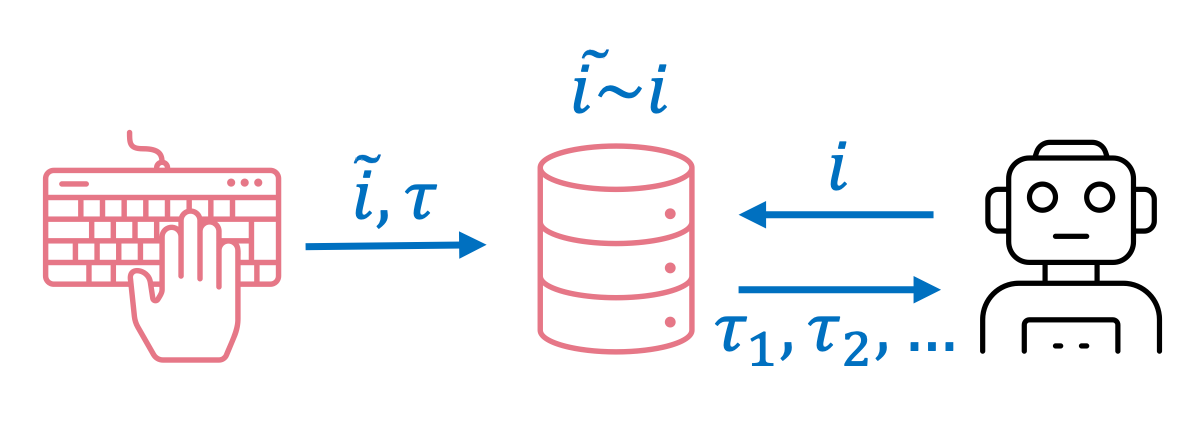
\includegraphics[width=0.7\linewidth]{figures/few_shot_2.png}
    \caption{Semantic search.}
    \label{fig:few_shot_2}
  \end{subfigure}
  \hfill
  \begin{subfigure}{0.49\linewidth}
  \centering
    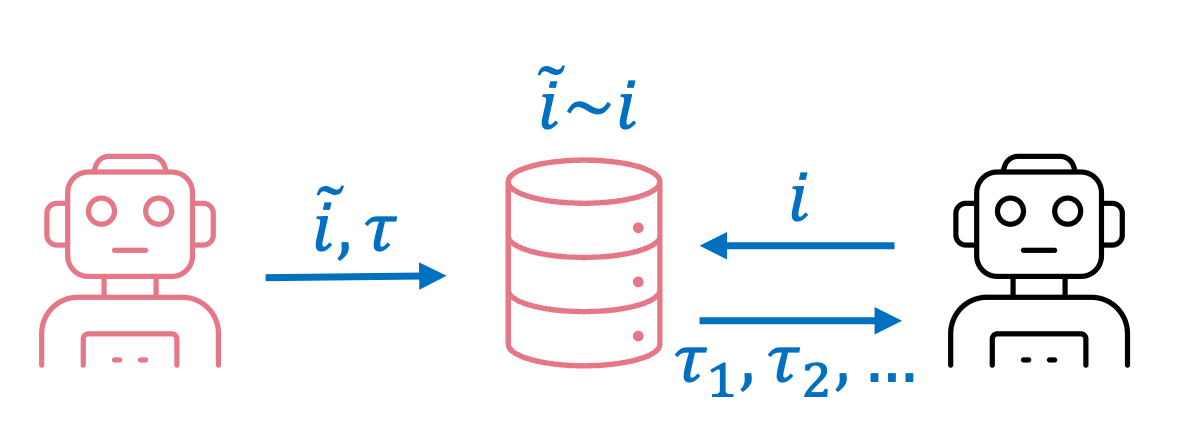
\includegraphics[width=0.7\linewidth]{figures/few_shot_3_n.png}
    \caption{Auxiliary model.}
    \label{fig:few_shot_3}
  \end{subfigure}
  \hfill
  \begin{subfigure}{0.49\linewidth}
  \centering
    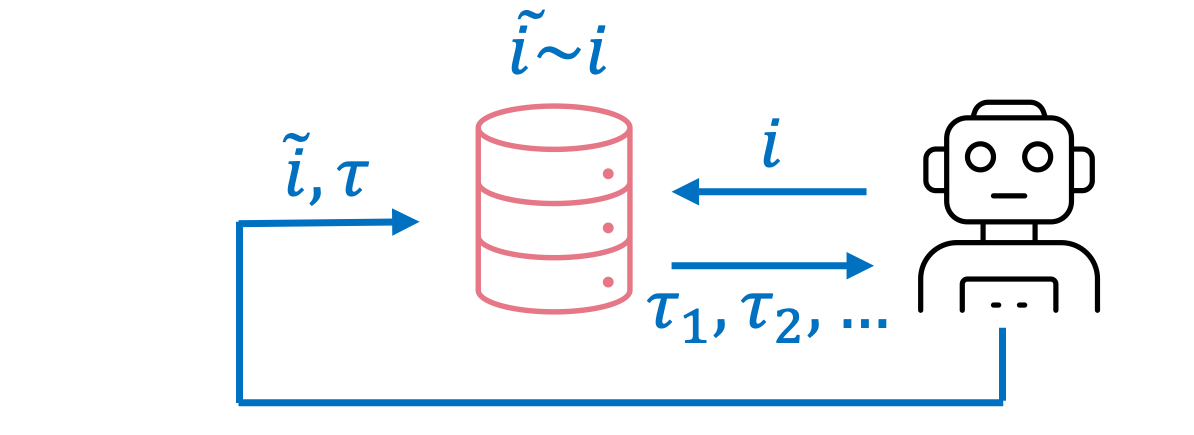
\includegraphics[width=0.7\linewidth]{figures/few_shot_4_n.png}
    \caption{Agent collected.}
    \label{fig:few_shot_4}
  \end{subfigure}
    \caption{The four most common few-shot learning strategies for ACUs.}
    \Description{
    This figure presents four common few-shot learning strategies for ACUs, each visualized through schematic subfigures involving a human (keyboard icon), an ACU (robot icon), and a demonstration store (cylinder icon). Arrows denote the direction and type of information flow, such as instructions $i$ and task demonstrations $\tau$, highlighting distinctions in data provenance and retrieval mechanisms. In (a) \emph{human-crafted}, the human directly provides demonstrations $\tau$ conditioned on $i$ to the agent. In (b) \emph{semantic search}, the human contributes $\tau$ and $i$ to a database, which the agent then queries bidirectionally to retrieve demonstrations. In (c) \emph{auxiliary model}, an auxiliary agent, rather than a human, populates the database with $\tau$ and $i$, while the main agent retrieves data as in (b), visually distinguishing the source of data via the origin of the arrows. In (d) \emph{agent collected}, the ACU both generates and retrieves demonstrations, forming a closed-loop interaction absent in other strategies and not explicitly detailed in the main text. These diagrams emphasize that although the textual descriptions may appear similar, the strategies differ fundamentally in terms of data origin and control flow.
}
    \label{fig:few_shot}
\end{figure}

\paragraph{Episodic Improvement through Planning} \label{sec:episodic_planning}

ACUs are goal-driven and often require planning to fulfill complex instructions $i$ \citep[Chapter~2.4]{russell_artificial_2022}. Most specialized agents perform implicit planning in their latent space, a process \citet{li_zero-shot_2023} called \emph{iterative planning}, where future states or action consequences are not explicitly constructed.

Agents based on foundation models typically generate explicit plans in text form. One common method is \emph{chain-of-thought} prompting \citep{liu_chain_2023}, which guides the model to produce intermediate reasoning steps before deciding on an action, improving the agent's performance \citepeg{rawles_android_2023, zhang_android_2024}. Another method involves decomposing an instruction into sequential sub-tasks, such as breaking down the task \texttt{Book an economy class flight from Hangzhou to Beijing} into steps like \texttt{Open the Alipay app} and \texttt{Input ``Hangzhou'' as the departure city} \citep{guan_intelligent_2023}. 

Plans can be refined iteratively.
For instance, after initial prompting, agents may either follow their initial plan rigidly \citepeg{kim_language_2023} or adapt it based on new observations \citepeg{sun_adaplanner_2023}.
Another refinement \citep{kim_language_2023} is done by prompting their foundation model to critique and refine its generated plans recursively. Although this can yield minor improvements, \citep{kambhampati_can_2024} argues that the benefits of self-critiquing may be limited.

These prompt-based planning strategies are considered informal planning, as they are based on the text output of foundation models, as opposed to internally simulating various action trajectories before deciding on one.
In contrast, formal planning can be implemented based on a search algorithm.
For instance, \citet{koh_tree_2024} simulate actions in a controlled environment and search through potential future states (observations) to better inform decision-making for the next action.
This approach shows significant performance gains, with task success rates improving by 50\% at a search depth of $5$. 
Building on this, \citet{chae_web_2024} fine-tune a model to predict the effects of actions on current observations, allowing for better decision-making without relying on an external simulator.
%Those ideas are similar to recent test-time compute techniques using agentic workflows \citep{snell2024scaling, singh2024enhancing}.



\subsubsection{Recommendations}
The landscape of learning strategies for ACUs is notably diverse.
Historically, RL and BC dominated as the primary paradigms. More recently, the emergence of foundation agents has shifted attention toward prompt-based learning. Despite this evolution, our analysis reveals that the field has yet to converge on a unified framework (see Appendix~\cref{fig:learning-strategy-dist}).

To enable a technology-agnostic characterization, we categorized learning paradigms into three sequential steps: pre-training, environment learning, and episodic improvement.
Our analysis reveals \textbf{a research gap in an effective and practical environment learning paradigm for foundation agents}:
Long-term memory approaches, while practical, often suffer from poor generalization. Storing raw trajectories is less beneficial than capturing underlying concepts, which remains highly challenging within this approach.
In contrast, reinforcement learning (RL) and behavioral cloning (BC) provide strong learning signals and enable concept abstraction, but they are highly resource-intensive, requiring either high-fidelity simulation environments or curated and labeled datasets for effective fine-tuning.

To address this bottleneck, we recommend research into the direction of introducing a \textbf{self-supervised fine-tuning stage between general pre-training and resource-intensive environment learning}. This intermediate stage would align general-purpose foundation models more closely to computer use contexts --- analogous to the role of RLHF in aligning LLMs with human preferences \citep{ziegler_fine_2020} or GRPO in improving reasoning \citep{shao2024deepseekmathpushinglimitsmathematical}. Such an alignment stage would equip models with domain-specific inductive biases, enabling faster and more robust adaptation during subsequent environment learning phases \citep{ouyang_training_2022}.

Our analysis also identifies planning as a major limitation in current ACU architectures. 
LLMs exhibit limited long-horizon planning capabilities \citep{valmeekam2023planning}, and the dynamics of the environment are often unknown, which hinders direct adaptation of symbolic approaches.
Thus, we argue that \textbf{planning in ACUs remains an open and pressing research challenge}. However, we identify two promising research directions for addressing this gap:
First, recent developments in reasoning-oriented LLMs, such as OpenAI o1, demonstrate promising capabilities in planning and long-horizon decision-making \citep{valmeekam2024llms, tan_towards_2024}. 
Adapting these capabilities for ACUs—and demonstrating robust planning performance in dynamic digital environments—is a critical next step.
Second, hybrid systems that combine symbolic planning with learned models of perception and action outcomes, such as those proposed by \citet{koh_tree_2024}, offer a compelling alternative. These methods draw from classical planning algorithms \citep[Chapter~11]{russell_artificial_2022} while leveraging neural components for generalization and flexibility.
% Forward state-space search could benefit from more agentic foundation models and approaches could adapt more sophisticated planning methods, such as using constraints \citep{porteous2001extraction,hoffmann2004ordered}.
Although these approaches extend beyond the ACU domain, we argue that ACUs provide an ideal testbed due to their complexity and fully digital nature. The integration of neuro-symbolic methods with agentic foundation models may pave the way for more sophisticated, adaptive, and general-purpose computer use agents.